\section{Benchmark Design}
\label{sec:design}

\subsection{Cohorts and Hourly Representation}

We use \MIMIC{} v3.1 and \EICU{} v2.0 \citep{johnson2023mimiciv,pollard2018eicu}. Common extraction and unit harmonization are based on RICU \citep{bennett2023ricu}. Each sample is one ICU stay with valid patient and stay metadata, ICU duration of at least 24 hours, and at least one observed time-series value in the first 24 hours. The processed cohorts contain 74,829 \MIMIC{} stays and 132,686 \EICU{} stays. We form their 207,515-stay union, \emph{Combined}, after schema compatibility checks and source-specific identifier namespacing. \MIMIC{}, \EICU{}, and \Combined{} are the three regimes; \Combined{} is pooled, not a separate cohort.

Each stay is represented as normalized values $x\in\mathbb{R}^{24\times84}$ and an observation mask $m\in\{0,1\}^{24\times84}$. Feature means and standard deviations are fitted on the training partition only. Missing cells are zero filled after normalization while $m$ preserves whether a value was observed. RICU aggregates repeated measurements within an hour by concept-specific rules, by default the median for numeric values and ``any'' for logical indicators, with exceptions such as summed urine output. The mask records whether at least one value fell in an hour, not how many, so within-hour sampling intensity is lost. The 84 retained variables are shared across regimes. Only 10.7\% to 15.3\% of tensor cells are observed, although most stays have at least one measurement in nearly every hour.

Patients are assigned to 70/15/15 train, validation, and test partitions for each seed. All stays for one patient remain in one partition. Task-specific missing labels are removed only after this assignment, and the same split is used for pretraining and downstream evaluation. Input normalization uses training data only. Direct length-of-stay variables, future-duration helpers, and derived features that expose downstream outcomes are excluded from the input.

\subsection{Endpoints and Horizons}

All tasks use the first 24 ICU hours as input. The endpoints follow task families of established ICU benchmarks \citep{harutyunyan2019multitask,van_de_water2024yaib}. They differ in prevalence, horizon, label construction, and target type, which can change an objective ranking. Classification uses area under the precision--recall curve (AUPRC), computed as average precision, because prevalence is low and endpoint dependent \citep{saito2015precisionrecall}. Mean test prevalence spans 1.6\%--20.3\% (\tableref{tab:test-support}). Twenty-four-hour mortality predicts death in hours 24--48. Hospital mortality predicts in-hospital death after hour 24. Deaths within the input window receive null labels. Creatinine-defined acute kidney injury (AKI) uses the minimum in hours 0--24 as baseline and seeks KDIGO stage~$\geq1$ evidence in hours 24--48: a later value at least 1.5 times baseline or at least 0.3 mg/dL above an earlier value within 48 hours \citepalias{kdigo2012aki}. Urine output is excluded. A missing baseline or forward measurement yields a null label. Remaining ICU length of stay (LOS) is ICU duration minus one day, clipped at zero. We retain this continuous target rather than impose a binary threshold. Absolute error keeps prediction misses interpretable in days.


\begin{figure*}[t]
\floatconts{fig:ssl-objectives}
{\caption{Core objective geometries. MAE reconstructs observed values at masked hours. JEPA's online encoder receives visible valid hours. Its EMA target encoder receives the full unmasked valid sequence. JEPA predicts layer-normalized, stop-gradient targets, with loss only on masked valid hours. Contrastive learning aligns projected pooled views. Auxiliary modules are discarded before downstream transfer.}}
{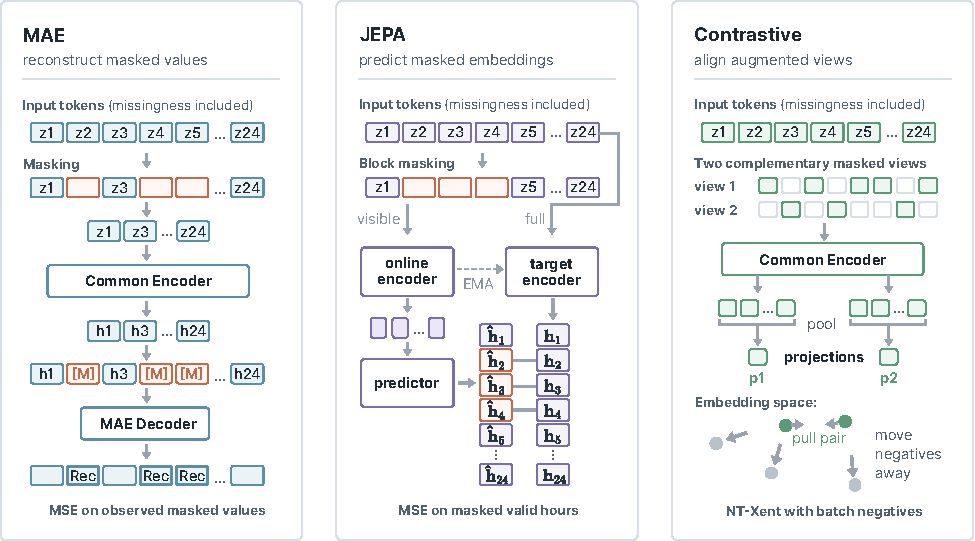
\includegraphics[width=\textwidth]{diagrams/fig04-ssl-objectives.pdf}}
\end{figure*}

\subsection{Shared Encoder and Objective-Specific Components}

Appendix Figure~\ref{fig:encoder-tokenization} shows the shared interface. Each hour is one continuous attention token: 84 normalized values and 84 observation indicators are concatenated and projected from $\mathbb{R}^{168}$ to $\mathbb{R}^{64}$, without value quantization or vocabulary lookup. The shared small Transformer has sinusoidal time encoding, two pre-layer-normalized layers, four heads, feed-forward width 256, and dropout .1. Empty hours are excluded from attention and SSL losses. Downstream heads mean-pool valid outputs. The same 159,808-parameter encoder transfers for every SSL method.

Figure~\ref{fig:ssl-objectives} contrasts the learning signals. \MAE{} masks random non-empty hours, encodes visible tokens, and uses a two-layer Transformer decoder to reconstruct observed normalized values at masked hours. Missing cells do not enter the loss. \JEPA{} masks up to three contiguous blocks. An online encoder and predictor estimate layer-normalized embeddings from a stop-gradient exponential-moving-average target encoder. Contrastive learning makes two complementary masked views, encodes each separately, mean-pools visible hours, and applies an MLP projection with an NT-Xent instance loss at temperature .07. Only the common encoder transfers downstream.

The implementations preserve reconstruction, latent prediction, and view agreement as distinct learning signals while sharing inputs, transferred encoder, and evaluation. Forecasting objectives are out of scope. Objective-specific masks and auxiliary modules retain each method's learning structure. MAE has 269,460 trainable pretraining parameters, JEPA has 189,440 plus a non-trainable 159,808-parameter target copy, and contrastive learning has 193,408 with two encoder passes. These are comparisons of complete implementations, not causal loss-function effects. Appendix Tables~\ref{tab:pretraining} and~\ref{tab:objective-details} summarize the pretraining contract and modules.
